\chapter{Конструкторская часть}
\label{cha:design}

\section{Требования к программе}

Программа должна предоставлять следующие возможности.

\begin{enumerate}
	\item Визуализацию сцены.
	\item Запуск системы.
	\item Останов системы.
\end{enumerate}

\section{Полигональная сетка}

Для работы с трехмерными объектами, удобно использовать полигональную сетку. Это позволяет получить реалистичное изображение, показать объем тела.
В разрабатываемом программном продукте использована треугольная полигональная сетка. Выбор треугольной полигональной сетки обосновывается следующими причинами:

\begin{enumerate}
	\item Разбиение тел на треугольники упрощает рендеринг, так как треугольник является выпуклой фигурой, а многие алгоритмы работают именно с выпуклыми полигонами 
	\item Любой многоугольник может быть разбит на некоторое количество треугольников 
	\item Невырожденный треугольник всегда расположен в одной плоскости, к нему легко восстановить нормаль
\end{enumerate}


\begin{figure}[ht!]
	\centering{
		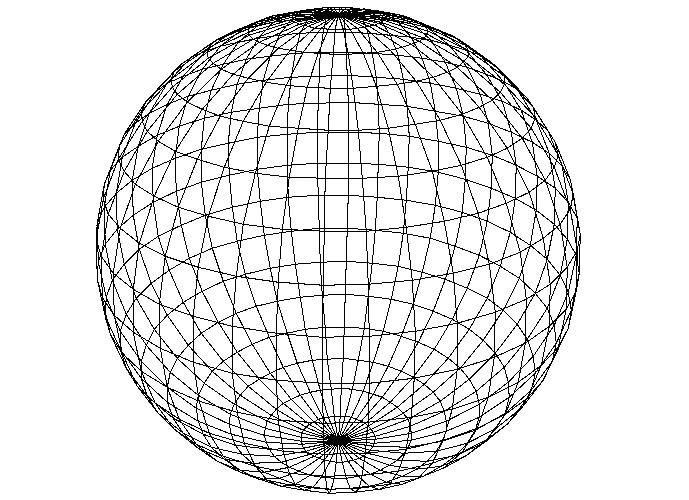
\includegraphics[width=1\textwidth]{planet.jpg}
		\caption{Пример полигональной сетки, изображающей планету}
		\label{ref:Warnock}}
\end{figure}

\subsection {Построение полигональной сетки}

Для построения полигональной сетки тел вращения используется следующий алгоритм.
Задается количество разбиений основания тела вращения и количество разбиений по высоте. Затем вычисляется угол, на который необходимо каждый раз поворачивать радиус-вектор основания, чтобы получить необходимое количество треугольников:

\begin{equation}
	angle = \frac{2 * \pi}{n * \phi}	,
\end{equation} 

где n * $\phi$ - число секторов на которые делится основание.


Основание тела при его создании лежит в плоскости xOz, поэтому координаты точек окружности, которые послужат вершинами треугольников, вычисляются следующим образом:
\begin{multline}
	\\
	x = x_0 + R * \cos(angle * i)\\
	y = y_0\\
	z = z_0 + R * \sin(angle * i) \\ ,
\end{multline}

где R - радиус основания вращения, i - номер итерации цикла, на котоом находится очередная точка.

\begin{figure}[ht!]
	\centering{
		\includegraphics[width=0.5\textwidth]{poly1.png}
		\caption{}
		\label{ref:Warnock}}
\end{figure}


Затем, зная зависимость радиуса от высоты, аналогичным способом проставляются точки на уровнях тела вращения с шагом:
\begin{equation}
	dh = \frac{yTop - yBottom}{heightSegments}
\end{equation}
где yTop - координата Y центра верхнего основания, yBottom - координата Y центра нижнего основания, heightSegments - число разбиений тела по высоте.

Затем  все полученные точки соединяются в четырехугольники. Точка соединяется с соседней сверху, соседней справа и точкой, которая лежит выше по диагонали справа. Таким образом, тело оказывается разделенным на четырехугольники. Затем  в каждом четырехугольнике проводится диагональ, и тело оказывается покрытым треугольной полигональной сеткой.

Этот алгоритм подходит для триангуляции цилиндра, конуса, усеченного конуса.

Чтобы разбить на треугольники сферу, необходимо разбить ее на усеченные конусы, а затем каждый из конусов триангулировать по описанному выше алгоритму.


\section{Вычисление интенсивности освещения в вершинах треугольника}
Для вычисления интенсивностей в вершинах треугольника сначала были вычислены нормали к его вершинам с учетом нормалей прилегающих к нему треугольников.
\begin{figure}[ht!]
	\centering{
		
\includegraphics[width=0.5\textwidth]{light.jpg}
		\caption{Нахождение нормалей к вершинам треугольника}
		\label{ref:Warnock}}
\end{figure}

\begin{equation}
	N_a = \frac{N_1 + N_2 + N_3}{3}
\end{equation}

Затем были найдены векторы от источника освещения к вершинам треугольника и углы между этими векторами и нормалями к каждой из вершин. 
Далее, интенсивность вычислялась по формуле:

\begin{equation}
	I[i] = angleCos[i] * source.GetI() + constLight ,
\end{equation}

где I[i] – интенсивность в i-й вершине треугольника, angleCos[i] – косинус угла между вектором от источника освещения к i-й вершине и нормалью к этой вершине, source.GetI() – интенсивность источника освещения, constLight - интенсивность рассеянного света, подобранная опытным путем.

Если в результате вычисления получалась интенсивность меньшая, чем constLight или большая, чем 1, значение корректировалось до constLight или 1 соответственно.




\section{Реализация метода Гуро с использованием Z-буфера}

Так как все тела, используемые в программе, были триангулированы, алгоритм закраски Гуро реализован для закраски треугольника. Для решения задачи удаления невидимых линий перед закраской координата Z каждого пиксела сравнивается со значением в буфере глубины, после этого принимается решение о необходимости закрашивать данный пиксел.

Для того чтобы при отрисовке выводить меньше пикселей, которые в дальнейшем будут перекрашены, было принято решение отсортировать треугольники по возрастанию по координате Z. Критерием сортировки является среднее значение координаты Z трех вершин треугольника. Такой подход позволяет сначала вывести на канву большую часть видимых треугольников, а затем при проверке не отрисовывать невидимые части треугольников, лежащих дальше от наблюдателя. Так как операция высвечивания пиксела занимает довольно много времени, такой подход должен ускорить процесс получения изображения.

Предварительно вершины треугольника сортируются по возрастанию их координат Y.

Поясняющий рисунок, на котором обозначены используемые в алгоритме обозначения:
\begin{figure}[ht!]
	\centering{
		\includegraphics[width=0.7\textwidth]{guro_z_buffer_pic_1.png}
		\caption{Поясняющий рисунок, на котором обозначены используемые в алгоритме обозначения:}
		\label{ref:Warnock}}
\end{figure}

Ниже представлен алгоритм закраски.

\begin{enumerate}
	\item Вычислить интенсивности в вершинах треугольника.
	\item Рассчитать изменение координаты Z в зависимости от Y.
	\item Цикл по сканирующим строкам от вершины с минимальным значение Y до вершины со средним значением Y.
	\item Определить координаты X левой и правой точек пересечения сканирующей строки со сторонами треугольника.
	\item Вычислить интенсивность в точках, найденных в пункте 4. Расчет для левой точки выполняется по следующей формуле: \begin{equation}
		I = (1 - (\frac{len2}{len1})) * points[0].I + (\frac{len2}{len1}) * points[1].I ,
	\end{equation} 
	
	где len2 – расстояние по Y от сканирующей строки до вершины с минимальным Y, len1 – длина стороны, на которой лежит точка, points[0].I – интенсивность в вершине с минимальным Y, points[1].I - интенсивность во второй вершине этой же стороны.
	Аналогичным образом рассчитывается интенсивность в правой точке сканирующей строки.
	\item Вычислить координаты Z крайних точек сканирующей строки по формулам: \begin{multline} \\
		z_{left} = point1.getZ() + dz_{12} * (y - point1.getY()); \\ 
		z_{right} = point1.getZ() + dz_{13} * (y - point1.getY()); \\
	\end{multline}
	$z_{left}$ и $z_{right}$ – координаты Z левой и правой точек пересечения сканирующей строки со сторонами треугольника, point1 - вершина с минимальным Y, $dz_{12}$ и $dz_{13}$ – изменение координат Z при смещение на 1 по Y для сторон треугольника, соединяющих вершины с минимальным и средним значением Y и вершины с минимальным и максимальным значением Y соответственно.

	\item Вычислить изменение координаты Z при смещении по X по сканирующей строке по формуле:
	\begin{equation}
		dzx = \frac{z_{right} - z_{left}}{end - start} ,
	\end{equation}

	где dzx – изменение координаты Z, $z_{right}$ и end – координаты Z и X правой крайней точки сканирующей строки, $z_{left}$ и start – координаты Z и X левой крайней точки сканирующей строки.

	\item Цикл по X от start до end по сканирующей строке.
	\item Проверить, не лежат ли координаты X и Y рассматриваемой точки за пределами канвы.
	\item Рассчитать координату Z рассматриваемой точки:
	\begin{equation}
		z = z_{left} + dzx * (x - start) ,
	\end{equation}
	
	где x и z – координаты точки, рассматриваемой на данной итерации.

	\item Сравнить полученную координату Z со значением в буфере глубины. Если найденная координата Z меньше значения в буфере глубины, то
	\item Поместить координату Z в буфер глубины.
	\item Вычислить параметр изменения интенсивности:
	\begin{equation}
		iP = (1 - \frac{lenQP}{lenQR}) * iQ + \frac{lenQP}{lenQR} * iR
	\end{equation}
	где iP – вычисляемый коэффициент, iQ и iR – значения интенсивностей в левой и правой точках сканирующей строки соответсвенно, lenQP и lenQR – расстояния от рассматриваемой точки до левой и правой точек сканирующей строки соответственно.
	
	\item Занести в буфер цвета пиксела с его базовым цветом, каждая компонента которого умножена на полученный коэффициент iP.
	\item Конец условия п.11
	\item Конец цикла п.8
	\item Конец цикла п.3
	\item Провести аналогичные действия для части треугольника, лежащей между вершиной со средним и максимальным значениями координаты Y.
\end{enumerate}



\section{Выбор используемых типов и структур данных}

В данной работе нужно будет реализовать следующие типы и структуры данных.

\begin{enumerate}
	\item Точка -- хранит положение, задается координатами x, y, z.
	\item Вектор -- хранит направление, задается x, y, z.
	\item Цвет -- вектор из трех чисел (синий, красный, зеленый).
	\item Планета -- хранит радиус, цвет и центр планеты.
	\item Ракета -- вектор из координат, описывающих ракету.
	\item Сцена -- список объектов, заданных планетой и ракетой.
	\item Источник света -- положение и направление света.
\end{enumerate}

\section{Вывод}

В данном разделе были описаны требования к программе, подробно рассмотрены алгоритмы z-буффера и закраски Гуро,
описаны типы и структуры данных, которые будут реализованы. Также рассмотрен способ вычисления интенсивности освещения и построения полигональной сетки.
